\chapter{Testes}
\label{cha:Testes}

Afim de satisfazer todos os requisitos descritos no capítulo \ref{cha:Requisitos}, foram efetuados testes do sistema e algoritmo durante toda a fase de desenvolvimento. Esses testes eram efetuados de maneira não estruturada, apenas para testar todos os possíveis casos de erro. Foi considerada a metodologia de \textit{Desenvolvimento orientado a testes}, que planeja o desenvolvimento primeiro de testes unitários e de integração, para depois o desenvolvimento da aplicação em si. Porém, a implantação dessa metodologia costuma aumentar consideravelmente o tempo de desenvolvimento de aplicações, por isso ela não foi implementada.

Por não ter testes unitários ou de integração, o desenvolvimento precisou ser meticuloso. Por isso, optou-se por utilizar Typescript na interface, um superconjunto de Javascript, o que significa que suporta a sintaxe de Javascript e suas funcionalidades, mas introduz outras funcionalidades, que no caso são os tipos. Esses tipos permitem analisar o código em tempo de compilação, exibindo-os durante o processo de desenvolvimento, tornando o código mais resistente a falhas. Do mesmo modo, nos microserviços implementados em Python foram usados a sintaxe de tipos, pela mesma vantagem. Python é uma linguagem dinâmica em que os tipos não são necessários, mas foram utilizados para trazer mais segurança. Por último, a API foi implementada em Go, uma linguagem compilada \textit{fortemente tipada}, o que significa que todas as variáveis possuem um tipo específico.

O trecho de código \ref{cod:sql-algoritmo} exibe a consulta ao banco para coletar os parâmetros de entrada do algoritmo. É possível observar que a consulta procura através das tabelas \verb|disciplinas| e \verb|turmas|, procura na tabela \verb|semestres| (que contém as disciplinas dos currículos), procura nas tabelas de avaliações, procura na tabela \verb|historicos| e utiliza-se de um filtro com as disciplinas e turmas já escolhidas pelo aluno, satisfazendo os requisitos RF01, RF02, RF03, RF04 e RF05. A fórmula matemática satisfaz o requisito RF06. Portanto, todos os requisitos funcionais do algoritmo foram satisfeitos. 

Como a implementação do algoritmo é um modelo matemático, pode-se observar que o requisito RNF2 (que determina que o algoritmo deve retornas os mesmos resultados para as mesmas entradas) é satisfeito. 

Foram efetuados testes de performance para verificar se os requisitos RNF1 e RNF3 foram satisfeitos. A figura \ref{fig:teste-performance} representa um teste de performance, com 40 usuários simultâneos autenticados solicitando recomendações diferentes a cada 1-5 segundos. É possível observar que o tempo médio de resposta das recomendações foi 20 milisegundos, e não houve nenhuma falha no sistema ou algoritmo. O teste de performance foi desenvolvido usando o framework \textit{Locust} \cite{site-locust}, utilizando a linguagem Python.

\begin{figure}[ht]
    \begin{center}
    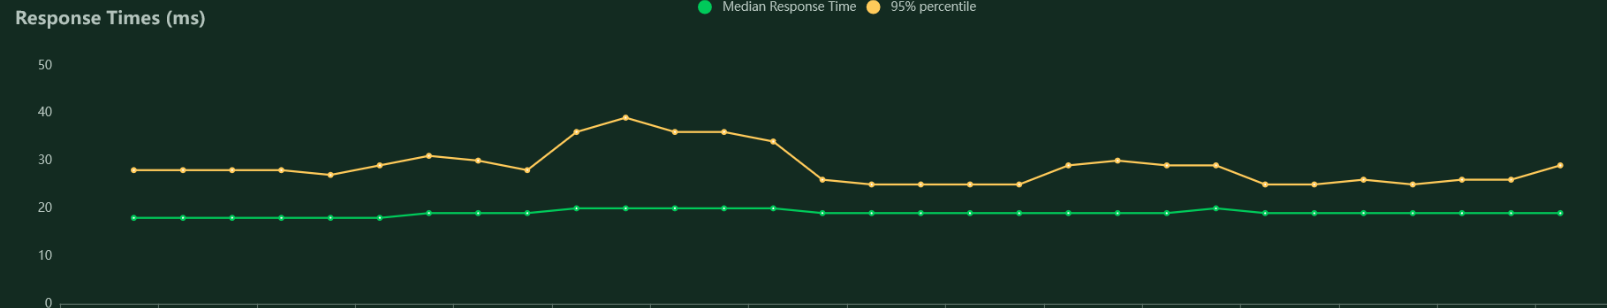
\includegraphics[width=390pt]{figuras/teste-performance.png}
    \caption{Teste de performance da recomendação}
    \label{fig:teste-performance}
    \end{center}
\end{figure}

Para satisfazer os requisitos do sistema, a interface e a API precisam agir de forma integrada. A lista abaixo contém os requisitos do sistema, o(s) componente(s) que os satisfazem, e a rota da API que é utilizada para alimentar a interface.

% \begin{table}[!ht]
%     \begin{center}
%         \begin{tabular}{ | m{0.1\textwidth} | m{0.4\textwidth} | m{0.4\textwidth} | }
%             \hline
%             Requisito & Componente(s) da interface & Rota(s) da API\tabularnewline\hline\hline
            
%             \textbf{RF07} & 
%             \verb|grade/+page.svelte| & 
%             \textit{/pesquisa/info}, \textit{/pesquisa/podecursar}, \textit{/pesquisa/faltacursar}, \textit{pesquisa/cursadas} e \textit{/disciplinas/info}
%             \tabularnewline\hline

%             \textbf{RF08} & 
%             \verb|HistoricoPopup.svelte| & 
%             \verb|/historico|
%             \tabularnewline\hline

%             \textbf{RF09} & 
%             Componentes em \verb|components/grade/turma| & 
%             \verb|/disciplinas/info|
%             \tabularnewline\hline

%             \textbf{RF10-12} & 
%             \verb|JanelaSalvar.svelte| e \verb|GrupoBotoes.svelte| & 
%             \verb|/grade|
%             \tabularnewline\hline

%             \textbf{RF13-14} & 
%             \verb|CheckLogin.svelte| e \verb|LoginPopup.svelte| & 
%             \verb|/login| e \verb|/logout|
%             \tabularnewline\hline

%             \textbf{RF15} & 
%             \verb|avaliacao/+page.svelte| & 
%             \verb|/avaliacoes/|
%             \tabularnewline\hline

%             \textbf{RF16-18} & 
%             \verb|CampoAvaliacao.svelte| & 
%             \verb|/avaliacoes/disciplina| e \verb|/avaliacoes/professor| 
%             \tabularnewline\hline
%         \end{tabular}
%     \end{center}
%     \caption{Implementação dos requisitos do sistema}
%     \label{tab:impl-sistema}
% \end{table}


\begin{itemize}
    \item \textbf{RF07:} O sistema deve permitir que o usuário crie uma grade horária para o próximo período.
    \begin{itemize}
        \item \textbf{Interface:} \verb|grade/+page.svelte|
        \item \textbf{API:} \verb|/pesquisa/{info,podecursar,faltacursar,cursadas}|
    \end{itemize}
    
    \item \textbf{RF08:} O sistema deve permitir que o usuário submita seu histórico escolar.
    \begin{itemize}
        \item \textbf{Interface:} \verb|HistoricoPopup.svelte|
        \item \textbf{API:} \verb|/historico|
    \end{itemize}

    \item \textbf{RF09:} O sistema deve permitir que o usuário selecione turmas das disciplinas para compor sua grade horária.
    \begin{itemize}
        \item \textbf{Interface:} Componentes em \verb|components/grade/turma|
        \item \textbf{API:} \verb|/disciplinas/info|
    \end{itemize}

    \item \textbf{RF10:} O sistema deve permitir que o usuário armazene a sua grade horária finalizada.
    \begin{itemize}
        \item \textbf{Interface:} \verb|JanelaSalvar.svelte| e \verb|GrupoBotoes.svelte|
        \item \textbf{API:} \verb|/grade|
    \end{itemize}

    \item \textbf{RF11:} O sistema deve permitir que o usuário compartilhe a sua grade horária finalizada.
    \begin{itemize}
        \item \textbf{Interface:} \verb|JanelaSalvar.svelte|
        \item \textbf{API:} \verb|/grade|
    \end{itemize}

    \item \textbf{RF12:} O sistema deve permitir que o usuário recupere uma grade horária montada a partir de um link compartilhado.
    \begin{itemize}
        \item \textbf{Interface:} \verb|grade/+page.svelte|
        \item \textbf{API:} \verb|/grade|
    \end{itemize}

    \item \textbf{RF13:} O sistema deve permitir que o usuário inicie uma sessão autenticada utilizando sua matrícula.
    \begin{itemize}
        \item \textbf{Interface:} \verb|CheckLogin.svelte| e \verb|LoginPopup.svelte|
        \item \textbf{API:} \verb|/login|
    \end{itemize}

    \item \textbf{RF14:} O sistema deve permitir que o usuário finalize uma sessão autenticada.
    \begin{itemize}
        \item \textbf{Interface:} \verb|LoginHeader.svelte|
        \item \textbf{API:} \verb|/logout|
    \end{itemize}

    \item \textbf{RF15:} O sistema deve permitir que o usuário avalie uma disciplina.
    \begin{itemize}
        \item \textbf{Interface:} \verb|avaliacao/+page.svelte|
        \item \textbf{API:} \verb|/avaliacoes/|
    \end{itemize}

    \item \textbf{RF16:} O sistema deve permitir que o usuário avalie um professor de uma disciplina.
    \begin{itemize}
        \item \textbf{Interface:} \verb|CampoAvaliacao.svelte|
        \item \textbf{API:} \verb|/avaliacoes/professor| 
    \end{itemize}

    \item \textbf{RF17:} O sistema deve permitir que o usuário altere uma avaliação feita anteriormente.
    \begin{itemize}
        \item \textbf{Interface:} \verb|CampoAvaliacao.svelte|
        \item \textbf{API:} \verb|/avaliacoes/disciplina| 
    \end{itemize}
\end{itemize}